\section{Introduction}
\label{sec:introduction}
Deterministic tractography algorithms~\cite{mori2002fiber} can
reconstruct white matter fiber tracts as a set of \emph{streamlines},
also known as \emph{tracks}, from diffusion Magnetic Resonance Imaging
(dMRI)~\cite{basser1994diffusion} data. A
streamline is a mathematical approximation of thousands of neuronal
axons expressing anatomical connectivity between different areas of
the brain, see Figure~\ref{fig:streamlines}. Recently there has been
an increase of attention in analysing dMRI/tractography data by means
of machine learning and pattern recognition methods,
e.g.~\cite{zhang2008identifying,wang2011tractography}. These methods often
require the data to lie in a vectorial space, which is not the case
for streamlines. Streamlines are polylines in $3$D space and have
different lengths and numbers of points. The goal of this work is to
investigate the features and limits of a specific Euclidean embedding,
i.e. the dissimilarity representation, that was recently applied to
the analysis of tractography data~\cite{olivetti2011supervised}.

The dissimilarity representation is an Euclidean embedding technique
defined by selecting a set of objects (e.g. a set of streamlines)
called \emph{prototypes}, and then by mapping any new object (e.g. any
new streamline) to the vector of distances from the prototypes. This
representation~\cite{pekalska2002generalized,balcan2008theory,chen2009similarity}
is usually presented in the context of classification and clustering
problems. It is a \emph{lossy} transformation in the sense that some
information is lost when projecting the data into the dissimilarity
space. To the best of our knowledge this loss, i.e. the degree of
approximation, has received little attention in the
literature. In~\cite{pekalska2006prototype} the approximation was
studied to decide among competing prototype selection policies only
for classification tasks. In this work we are interested in assessing
and controlling this loss without restriction to the classification
scenario.

This work is motivated by practical applications about executing
common algorithms, like spatial queries, clustering or classification,
on large collections of objects that do not have a natural vectorial
space representation. The lack of the vectorial representation avoids
the use of some of those algorithms and of computationally efficient
implementations. The dissimilarity space representation could be the
way to provide such a vectorial representation and for this reason it
is crucial to assess the degree of approximation introduced. Besides
this characterisation we propose the use of a stochastic approximation
of an optimal algorithm for prototype selection that scales well on
large datasets. This scalability issue is of primary importance for
tractographies given that a full brain tractography is a large
collection of streamlines, usually $\approx 3 \times 10^5$, a size for
which algorithms may become impractical. We provide practical
examples both from simulated data and human brain tractographies.

\begin{figure}
  \centering
  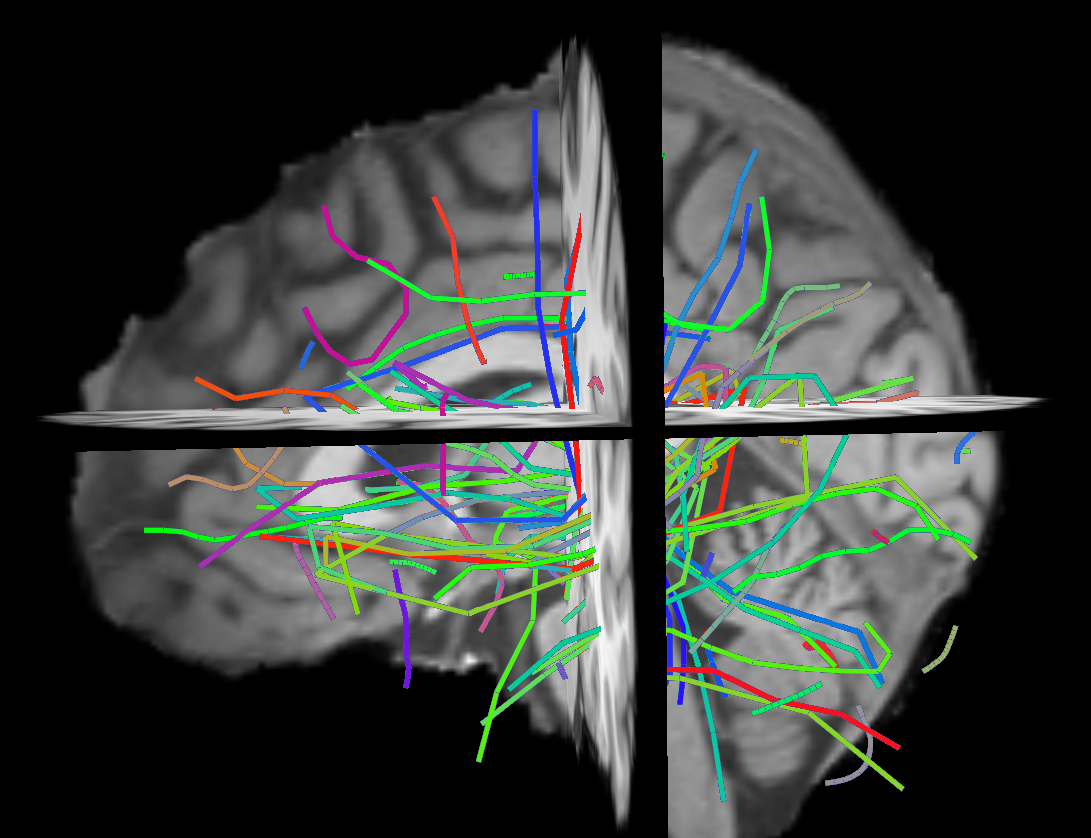
\includegraphics[width=5.0cm]{prni2012b.png}
  \caption{A set of $100$ streamlines, i.e. an example of prototypes,
    from a full tractography}
  \label{fig:streamlines}
\end{figure}

%%% Local Variables: 
%%% mode: latex
%%% TeX-master: "nguyen_dissimilarity"
%%% End: 

